\documentclass[journal]{./IEEE/IEEEtran}
\usepackage{graphicx,float,caption,multicol,multirow}

\captionsetup{labelfont=bf,singlelinecheck=false,
              labelsep=space,skip=2pt}
\setlength{\abovecaptionskip}{15pt plus 3pt minus 2pt}

\newcommand{\SPTITLE}{PANG-KAT: A Dedicated Tokenizer for the Tagalog Language}
\newcommand{\ADVISEE}{Justin Louis L. Saavedra}
\newcommand{\ADVISER}{Jaderick P. Pabico}

\newcommand{\BSCS}{Bachelor of Science in Computer Science}
\newcommand{\ICS}{Institute of Computer Science}
\newcommand{\UPLB}{University of the Philippines Los Ba\~{n}os}
\newcommand{\REMARK}{\thanks{Presented to the Faculty of the \ICS, \UPLB\
                             in partial fulfillment of the requirements
                             for the Degree of \BSCS}}
        
\markboth{2025 ICS Undergraduate Research Symposium}{}
\title{\SPTITLE}
\author{\ADVISEE~and~\ADVISER%
\REMARK
}
\pubid{\copyright~2025~ICS \UPLB}
\pagenumbering{gobble}

\usepackage[sorting=none]{biblatex}
\addbibresource{saavedra-ieee.bib}

%%%%%%%%%%%%%%%%%%%%%%%%%%%%%%%%%%%%%%%%%%%%%%%%%%%%%%%%%%%%%%%%%%%%%%%%%%

\begin{document}

% TITLE
\maketitle

% ABSTRACT
\begin{abstract}
Tokenization is a critical preprocessing step in many natural language processing (NLP) tasks, yet most general tokenization methods do not effectively recognize the unique grammatical features, named entities (NEs), and multi-word expressions (MWEs) of a language. These issues are more evident for low-resource languages, including the Tagalog language, which is further complicated by code-switching. Thus, this study introduces PANG-KAT, a hybrid rule and dictionary-based tokenizer dedicated to Tagalog that is designed to handle these aforementioned challenges for both short- and long-term unit tokenization. Performance evaluation results indicate good performance with F1 scores of 0.9518 and 0.9130 on News-PH NLI dataset and F1 scores of 0.9624 and 0.9411 on articles from Pilipino Star Ngayon (May 2025) for short and longer unit tokenization, respectively. These results affirm the effectiveness of its rule set and dictionaries in capturing the patterns in Tagalog and Taglish texts.
\end{abstract}

% INDEX TERMS
\begin{keywords}
Tokenization, Tagalog, Tagalog-English, Named Entity Recognition, NLP
\end{keywords}

% INTRODUCTION
\section{Introduction}

\subsection{Background of the Study}

In the Philippines, the Tagalog language is the language spoken by 23 \% of the Philippine population, which represents the largest cultural-linguistic group in the country. Despite the cultural significance of Tagalog within the Philippines, several fundamental aspects of modern natural language processing (NLP) for processing the widely used language are underdeveloped. The scarcity of Tagalog data and its typological differences from other high-resourced Austronesian languages pose challenges for further computational exploration of the language in modern natural language processing {\cite{TweetTaglish}}. \\

Within the field of NLP, one crucial area in need of development for low-resource languages is tokenization {\cite{Cutter}}. Among these low-resource languages is the Tagalog language  {\cite{TweetTaglish}}. Tokenization is a primary step in modeling textual information, which involves breaking down a text into smaller units known as tokens {\cite{Cutter}}. The absence of suitable tokenizers for the Tagalog language stands as a significant obstacle that hinders the effective processing of its language resources {\cite{TweetTaglish}}. \\

Space tokenization is the common method used by NLP systems for token separation, which utilizes the space character as the primary character used as token boundaries. While this basic tokenizer, which splits text at space characters, demonstrates acceptable accuracy, it lacks the ability to identify unmarked token boundaries, leading to erroneous splitting, especially for tokens containing space characters {\cite{Cutter}}. This issue is prominent when dealing with named entities (NEs) in texts, which are nouns specific to a particular language or domain {\cite{ChemTok}}. Furthermore, simple space tokenization also fails to accurately capture unique multi-word expressions of a given language {\cite{Sudachi}}. \\

To address the issue regarding NEs, incorporating Named Entity Recognition (NER) during the tokenization process is a viable solution. NER is a preliminary step for information extraction, which identifies and categorizes proper nouns into predefined categories. In this context, an entity is considered an independent and distinct entity {\cite{ChemTok}}. The detection of named entities proves valuable in various NLP applications such as semantic analysis, information retrieval, and machine translation. Similar to NER, the recognition of multi-word expressions may also be incorporated during the tokenization process {\cite{Sudachi}}. \\

With the presence of numerous language-specific NEs and multi-word expressions, tokenization is regarded as a language-specific task. The challenge is compounded by the use of the same characters for different purposes across languages, and the complexity is further increased by the presence of code-switching or code-mixing {\cite{Cutter}}.  Code-switching is a sociolinguistic phenomenon, which involves the blending of two distinct languages within a single utterance or conversation {\cite{TweetTaglish}}. \\

In the Philippines, the prevalent use of code-switching between Tagalog and English, creating Taglish, became a cultural and societal norm, wherein Taglish is frequently viewed as the language of the "educated, middle- and upper-class urbanites of the Philippines," and individuals may code-switch to either align with or distance themselves from this identity.  Thus, effectively processing the language for real-world Tagalog applications necessitates not only a strong grasp of Tagalog but also a thorough understanding of the common behaviors related to Taglish code-switching {\cite{TweetTaglish}}. \\

\newpage

\subsection{Statement of the Problem}

Despite the cultural significance of Tagalog as the most spoken language in the Philippines, it lacks a suitable tokenizer for accurately processing its grammatical complexities and promoting further NLP advancements with its language resources. Therefore, this study seeks to develop a dedicated tokenizer for the Tagalog language to address the lack of a suitable tokenizer for the language. Additionally, the tokenizer will also include features for the recognition of Tagalog NEs and multi-word expressions. Furthermore, the tokenizer will be tested and refined for Taglish tokenization to improve its generalizability and usability for real-world Tagalog language processing applications.

\subsection{Objectives of the Study}

This study aims to develop a dedicated tokenizer for the Tagalog language, which would also incorporate the recognition of Tagalog NEs and multi-word expressions, and Taglish tokenization in an attempt to make a general tokenizer for real-world Tagalog language processing applications. \\

Specifically, to achieve the following objectives: \\

\begin{itemize}
  \item To create a dictionary containing Tagalog NEs and multi-word expressions to facilitate their recognition in the tokenization process. \\
  \item To annotate a Taglish corpus into pre-segmented tokens, to be used for assessing the adaptability of the Tagalog tokenizer on Taglish data \\
  \item To construct a hybrid rule and dictionary-based tokenizer for the Tagalog language \\
  \item To evaluate the tokenizer based on the following performance evaluation metrics:
    \begin{itemize}
        \item Accuracy
        \item Precision
        \item Recall
        \item F1-Score
    \end{itemize}
\end{itemize}

\subsection{Significance of the Study}

Tokenizers are primary tools responsible for the pre-processing of textual information for it to be understood and processed by more advanced natural language processing systems {\cite{Cutter}}. The significance of this study lies in the development of a dedicated tokenizer for the Tagalog language, which is the Philippines’ most widely spoken language, but lacks a suitable tokenizer that prevents its further computational exploration {\cite{TweetTaglish}}. \\

\newpage

Specifically, the result of the study is designed to benefit the following: \\

\subsubsection{Advancement of Tagalog language processing systems}

The absence of adequate tools and resources for processing Tagalog text impedes the progress of Tagalog language processing systems in the Philippines. This study seeks to bridge this gap through the development of a dedicated tokenizer for the Tagalog language, which lays the foundation for the development of more advanced Tagalog language processing systems capable of accurately analyzing and interpreting Tagalog text. \\

\subsubsection{Real-World applications} 

 The prevalent use of code-switching between the Tagalog and English languages in Filipino daily conversations necessitates the tokenizer to also be able to handle Taglish tokenization {\cite{TweetTaglish}}. By developing a dedicated Tagalog language tokenizer to also incorporate features for Taglish tokenization, this study seeks to improve the tokenizer’s capability and adaptability for real-world applications. \\

 \subsubsection{Supporting linguistic research and development}

 The development of a dedicated Tagalog tokenizer also contributes to the broader field of linguistics by providing insights into the structural and semantic characteristics of the language. This study seeks to enrich our understanding of Tagalog language patterns and usage, to encourage future research and development in both Tagalog linguistics and computational linguistics. \\

\subsubsection{Future researchers}

This study seeks to encourage further research in Tagalog natural language processing. Future researchers may utilize this study as a tested basis or guide when looking for related literature to reinforce the results of the study or for exploring related language-processing tasks. \\

\subsection{Scope and Limitations of the Study}

According to Gordon {\cite{TagalogVariants}}, there are eight major Tagalog dialects, namely,  Bataan, Batangas, Bulacan, Lubang, Manila, Marinduque, Tanay-Paete, and Tayabas-Quezon. Despite having differences in intonation and vocabulary among these variants, they remain mutually intelligible, which allows speakers of one to understand the others. In this study, the Tagalog tokenizer will concentrate on Manila Tagalog, as it is the most widely used and popular dialect, which served as the foundation for the development of the Filipino language. \\

\newpage

\section{Review of Related Literature}

This chapter contains literature and studies from both local and foreign settings, which are mostly gathered using Google and Google Scholar, to better understand the rationale and goals of the current research. It will focus on three subtopics, namely: natural language processing (NLP), tokenization, and approaches to developing tokenizers. Articles were selected for each subtopic based on their relevance in providing a comprehensive understanding of the research context.

\subsection {Natural Language Processing}

In 1957, Noam Chomsky laid the theoretical foundation for natural language processing (NLP) with his Phrase-Structure Grammar, which allowed the translation of natural language sentences into a format that can be understood by computers. The overall goal of this creation was to build a computer that could think and communicate like humans, which paved the way for the development of artificial intelligence. Nowadays, NLP has become an essential aspect of artificial intelligence, which enables computers to comprehend, interpret, and use human languages to achieve specific goals {\cite{NLPHist}}. \\

Language is an important medium that facilitates communication among humans. Through natural language processing (NLP), computers were not only able to understand human languages but also allowed the automated processing of human conversations, which can be used for retrieving information that can be used for higher-level NLP tasks. The advent of the Internet led to the exponential rise in daily human conversations available through online platforms.  These drastic changes emphasize the importance of NLP for leveraging computers to understand and derive information from these exchanges, and to propel further developments of NLP to improve its applications in addressing human problems. To identify what further advancements can be made in this field and evoke its continuous, improved development in the coming years, an assessment of the current state of NLP research is important {\cite{NLPInPH}}. \\

The general state of NLP research is commonly presented by general studies through systematic assessments using bibliometric reviews. However, these general studies often overlook scientific research from underrepresented regions that may include underrepresented languages, which is the case for the Philippines and its languages {\cite{NLPInPH}}. To address this gap, Roxas et al. {\cite{NLPInPH}} conducted a comprehensive analysis of NLP works in the Philippines, with the aim of providing a mapping of its scientific landscape and identifying research trends, focus areas, and research gaps that can be explored and developed by local researchers {\cite{NLPInPH}}. \\

The results of their study showed that there is a low number of NLP research publications in the Philippines over the 15-year investigation period of 2006 to 2020. Additionally, the predominantly identified language of investigation among the documents studied is English, followed by Tagalog and other Philippine languages. Moreover, a limited scope of research on NLP was observed among the documents, focusing mostly on text processing, classification and analysis, and sentiment analysis. Based on these identified research gaps, the researchers recommend expanding NLP research in the Philippines to include representation of other Philippine languages and the exploration of more NLP areas {\cite{NLPInPH}}. \\

Despite the recommendations for further expanding NLP research on Philippine languages, several fundamental aspects of modern NLP are inaccessible or insufficiently developed for these languages, which are considered low-resource languages. This problem is even persistent in the most widely spoken language of the country, which is the Tagalog language. This is due to the scarcity of Tagalog data and its typological differences from other high-resourced Austronesian languages, which pose challenges for further computational exploration of the language in modern NLP {\cite{TweetTaglish}}. \\

Although NLP tools developed for other languages can be used for processing Tagalog, their performance is inferior compared to tools specifically designed for the language. For instance, the study by Aquino and de Leon {\cite{Ugnayan}} that revolves around evaluating different methods for dependency parsing in low-resource languages, specifically the Tagalog language, showed that monolingual models outperform both cross-lingual and multilingual models in processing a target language, even with minimal available training data. \\

Dependency parsing is a process of analyzing the relationships between words in a sentence, used in various natural language processing and machine learning systems. In general, parsers perform best with high-resource languages and struggle with low-resource languages. To improve parsers' performance for low-resource languages, multi-lingual and cross-lingual approaches are introduced. However, these approaches require abundant training data from closely related languages, which is problematic for Tagalog due to its significant typological differences from other Austronesian languages {\cite{Ugnayan}}. \\

To address this issue, the researchers introduced a monolingual parsing approach that uses minimal training data from the Tagalog language to train the monolingual model. This approach is founded on several studies on Indian languages, indicating that monolingual models, even with minimal target language data, perform better than cross-lingual and multilingual models in processing the target language. This is because monolingual models can better capture the grammatical complexities of the target language. The target language's representation could also be less accurate if it has significant typological differences with its closely related languages {\cite{Ugnayan}}. \\

To test these findings for Tagalog, they developed Ugnayan, which is a Tagalog dependency treebank needed for testing the parsers' performance on Tagalog data and for training their monolingual model. The results of their study showed that the monolingual approach outperforms both cross-lingual and multilingual dependency parsing for the Tagalog language and affirmed that monolingual models outperform both cross-lingual and multilingual models in processing a target language, even with minimal available training data. This finding is significant in developing models for processing low-resource languages, such as the Tagalog language {\cite{Ugnayan}}. 

\subsection {Tokenization}

Within the field of NLP, one crucial area in need of development for low-resourced languages is tokenization, which is a primary step in modeling textual information that involves breaking down a text into meaningful, smaller units known as tokens {\cite{Cutter}}. To establish the importance of tokenization in NLP, Friendman {\cite{TokenizationInKnowledge}} generalized the concept of tokenization in understanding knowledge, not by treating it as a whole unit, but as a product of a combination of more basic elements. Different analogies on how tokens structure knowledge were explored, such as tokens representing the basic forms of matter that make up living organisms in nature, the smallest unit of information in scientific data, and the elementary instructions in math and logic. \\

The rationale of these analogies is to show that different forms of knowledge are composed of different elements built in different ways. Moreover, it uses analogies to draw parallels between these tokens and those utilized in deep learning systems (DLS) to power artificial intelligence, demonstrating how each perspective respectively deconstructs knowledge into its most basic components, suggesting the possibility of adapting these same principles in token modeling across different contexts {\cite{TokenizationInKnowledge}}. \\

This exploration is motivated by how DLS processes information like the brain's intricate decision-making power. The paper suggests that, similar to how the human brain processes knowledge across different fields by tokenizing them within specific contexts, DLS could benefit from adopting the same tokenization process for improved information extraction.  It emphasized the critical role of tokens’ quality in DLS, as these are essential in generating a coherent and accurate sequence of tokens that collectively form knowledge {\cite{TokenizationInKnowledge}}. \\

For instance, the study of Singh and Saini {\cite{TokenizationForIRS}} explored how current tokenization algorithms used in information retrieval systems (IRS) fail to efficiently and accurately retrieve relevant information housed by documents in their system due to inaccuracies in their token identification process. Porter's algorithm is the widely used tokenization algorithm in the IRS. However, its token identification process suffers from inefficiency and inaccuracy, consequently affecting the performance of the IRS {\cite{TokenizationForIRS}}. \\

\newpage

IRS is used for storing indexed documents and retrieving relevant information from them by locating them within the system using ranking or indexing algorithms based on a user's query. Documents ranked higher in this order are more likely to be relevant and useful for fulfilling the user's needs. These ranking or indexing algorithms rely on the output of tokenization algorithms as input. Thus, their performance is heavily dependent on the quality of tokens generated by the tokenization process, which emphasizes the significance of developing a new tokenizer with improved token identification accuracy {\cite{TokenizationForIRS}}. \\

To address this issue, they developed a new tokenizer with pre-processing to produce more accurate and effective tokens in an efficient manner compared to other traditional tokenization algorithms. Results of their study showed that the tokenizer provided improved token identification accuracy, which also enhances the overall accuracy of the IRS. Moreover, it reduces the number of tokens generated per document, leading to less storage space, which makes it easier to store and retrieve, thereby enhancing not only the accuracy but also the efficiency of the IRS {\cite{TokenizationForIRS}}. \\

This emphasized the advantages of having a dedicated tokenizer that suits the needs of a particular task or context, which is also the same as creating a dedicated tokenizer that could cater to the grammatical complexities of a specific language. This is particularly true for low-resource languages, such as the Tagalog language, as the absence of suitable tokenizers for the Tagalog language stands as a significant obstacle that hinders the effective processing of its language resources {\cite{TweetTaglish}}. Therefore, there is a need to create a dedicated tokenizer for the Tagalog language.

\subsection {Approaches to Developing Tokenizers}

Researchers in the field have employed different approaches in developing tokenization systems, including rule-based, dictionary-based, machine learning-based, and hybrid systems {\cite{ChemTok}}. \\

According to Graën et al. {\cite{Cutter}}, "there is a need for tokenizers that can be adapted to a particular language and text variants”. Moreover, specific tokenization requirements also arise for processing texts in certain domains, genres, or historical text variants. \\

To address this issue, they introduced Cutter, a rule-based tokenizer designed to be easily adaptable to different languages and their respective text variants. Currently, it supports the languages of Catalan, Dutch, English, French, German, Italian, Portuguese, Romansh, Spanish, and Swedish. To include support for a specific language, its language-specific token identification rules must be added to Cutter's rule set {\cite{Cutter}}. \\

\newpage

Cutter adopts a distinctive approach compared to basic tokenizers that treat text as a sequence of characters and make decisions about token boundaries on a local basis. Instead, it employs a sequential list of patterns created through advanced regular expressions to identify tokens recursively. This methodology enables it to consider long-distance relationships between characters, which is a crucial factor for precise tokenization in numerous languages {\cite{Cutter}}. \\

Cutter is characterized by its language independence and modularity. The fundamental rules of Cutter are not tied to a specific language, which facilitates the adaptation of the tokenizer to different languages. Its rule system is modular, which provides flexibility for the inclusion of new language-specific or domain-specific rules to broaden its language support capabilities {\cite{Cutter}}. \\

In modern times, machine learning approaches have predominantly replaced rule-based methods in NLP techniques, including tokenization, due to their ability to adapt to unforeseen scenarios through pattern abstraction. However, machine learning approaches are mostly suited only for high-resourced languages with abundant training data. Generating sufficient training data for low-resourced languages presents a considerable challenge, demanding considerable time and effort for researchers in the said field. In a different study conducted by Takaoka et al. {\cite{Sudachi}},  they developed Sudachi, a Japanese Tokenizer tailored for business applications. Sudachi aims to overcome the limitations of existing tokenizers for Japanese text, which lack the integrated features for recognizing both short and longer units, commonly known as named entities (NEs). They concluded that the integration of these features for a tokenizer is essential for specific business tasks, where short unit recognition is beneficial for search functionalities, and named entity recognition (NER) plays a crucial role in applications such as syntactic or semantic analysis and information retrieval. \\

To address this issue, Sudachi implemented a multiple-granularity tokenization approach, offering users the flexibility to specify the desired level of granularity for token separation, whether it be short units or longer units, depending on the specific needs of the task requiring tokenization. For accurate tokenization, Sudachi relies on a dictionary-based tokenization method. Their dictionary encompasses Japanese short units, multi-word expressions, NEs, and the shorter units comprising NEs. This ensures the generation of tokens with varied granularity tailored to each application's specific purpose. They also employed normalization to address variations in word notation, enhancing the consistency and accuracy of tokens by adding the normalized form of these variations into their dictionary {\cite{Sudachi}}. \\

\newpage

Takaoka et al. {\cite{Sudachi}} emphasized that while NER is not precisely a subject of tokenization, achieving accurate NER requires lexical information obtained through the tokenization process, which led to their decision to incorporate it into their tokenizer. Moreover, they concluded that integrating NER into the tokenization step is more efficient, particularly for dictionary-based tokenizers, which is achieved by incorporating NEs into the tokenizer's dictionary. This approach also enhances NER accuracy and enables the handling of multi-word expressions. \\

Tokenization techniques depend on the task's context and objectives. The simplest technique involves segmenting tokens using whitespaces. However, in technical domains, relying solely on space-based tokenization is inadequate and inappropriate due to various factors such as diverse and technical terminologies, inconsistent spacing, ambiguous punctuations, including punctuations within NEs, nonstandard orthography, and the continuous introduction of new vocabularies. In the biomedical and chemical/drug domain, existing tokenizers face difficulties in handling the distinct features of chemical-named entities, leading to imprecise tokenization that impedes subsequent NLP tasks in the said field {\cite{ChemTok}}. \\

To address this issue, Akkasi et al. {\cite{ChemTok}} developed ChemTok, a rule-based tokenizer specifically designed for the recognition and segmentation of chemical-named entities (NEs) using the Inside–Outside–Beginning (IOB) tagging within scientific texts. The rules employed by ChemTok were manually extracted from two comprehensive chemical/drugs datasets:  the BioCreative IV Critical Assessment of Information Extraction in Biology (ChemDNER) corpus and the SemEval 2013 Drug Name Recognition corpus. \\

The results of the study revealed that ChemTok demonstrated enhanced tokenization performance and improved accuracy in NER, especially for challenging categories such as abbreviations and systematic NEs. Moreover, the researchers concluded that ChemTok's rule-based approach could streamline its adaptability to different contexts and chemical subdomains {\cite{ChemTok}}. \\

Machine-learning-based tokenizers are primarily developed using supervised machine-learning algorithms, which require an adequate amount of training data with pre-segmented texts into tokens to determine token boundaries before further processing. The lack of prior knowledge regarding token and NE boundaries in these approaches may lead to inaccurate segmentation of NEs during the tokenization process {\cite{ChemTok}}. 

\newpage

\subsection {Synthesis}

The study of Roxas et al. {\cite{NLPInPH}} observed few NLP publications in the Philippines from 2006 to 2020, which were also predominantly focused on the English language and had limited scope in NLP research. Due to this, they recommended expanding NLP research in the country to include Philippine languages and broaden the range of NLP tasks to be explored by future researchers. However, this exploration of Philippine languages is hindered due to the lack of suitable NLP tools to effectively process its language resources {\cite{TweetTaglish}}, particularly a tokenizer that is a primary tool needed to accurately segregate text data into meaningful chunks that a computer can understand to facilitate its processing for higher-level NLP tasks {\cite{Cutter}}. \\

In the Philippines, the Tagalog language is the most widely spoken language in the country. However, despite its cultural significance, NLP tools to process the language remain underdeveloped due to the language being a low-resource language with inadequate data to propel its further development in the field of NLP {\cite{TweetTaglish}}. Although tokenization techniques designed for other languages can be employed for Tagalog resources, their performance is inferior and could lead to inaccurate segmentation of tokens because of their inability to detect the grammatical complexities of the Tagalog language. This is undesirable as the performance of higher-level NLP and artificial intelligence systems powered by deep learning is dependent on the quality of tokens produced by their prior tokenization technique {\cite{TokenizationInKnowledge}}. \\

Therefore, there is a need to develop a dedicated tokenizer for the Tagalog language. However, the scarcity of annotated Tagalog data {\cite{TweetTaglish}} poses a challenge for developing a machine learning-based tokenizer for the language, as this approach is mostly suitable only for high-resource languages with abundant training data {\cite{ChemTok}}{\cite{Cutter}}. Given this limitation, the researcher in the present study proposes an alternative approach involving a hybrid rule and dictionary-based tokenizer, named PANG-KAT. \\

PANG-KAT will employ rules for initial short-unit tokenization. Afterward, its accompanying dictionary will be utilized to reinforce the rules for longer unit tokenization and to incorporate the recognition of Tagalog-named entities and multi-word expressions in its tokenization process. These features were inspired by Sudachi {\cite{Sudachi}} to improve the general usability of the tokenizer. Lastly, inspired by Chemtok {\cite{ChemTok}} and Cutter {\cite{Cutter}}, the rule-based approach was employed to improve the tokenizer’s language independence and modularity, to streamline its adaptability, and make it also suitable for Tagalog-English (Taglish) tokenization. 

\newpage

\section{Methodology}

In this study, the researcher proposes to develop PANG-KAT, a hybrid rule and dictionary-based tokenizer for the Tagalog language. PANG-KAT aims to incorporate the recognition of Tagalog-named entities and multi-word expressions in its tokenization process. To achieve this, PANG-KAT will employ rules for initial short-unit tokenization. Afterward, its accompanying dictionary will be utilized to reinforce the rules for longer unit tokenization, producing more discriminative tokens such as named entities (NEs) and multi-word expressions (MWEs), which are useful for applications such as syntactic or semantic analysis and information retrieval {\cite{Sudachi}}. \\

\begin{figure}[H]
    \centering
    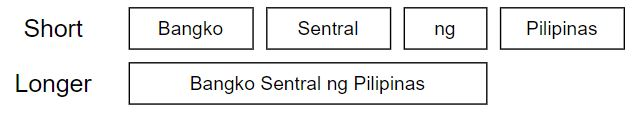
\includegraphics[scale=0.66]{images/Short and Longer Unit Tokenization.JPG}
    \captionsetup{justification=centering}
    \caption{An example of short and longer unit tokenization. In short unit tokenization, texts are tokenized into short parts. In contrast, for longer unit tokenization, texts are tokenized into more discriminative tokens such as Tagalog NE.}
\end{figure}

This approach is chosen instead of a machine learning approach due to the scarcity of various pre-annotated Tagalog corpora {\cite{TweetTaglish}} that can be used as training data for a machine learning model. Moreover, numerous studies suggest that comprehensive studies on general language typically necessitate an ideal corpus size of approximately a million tokens to sufficiently represent the low-frequency words in a language {\cite{corpusSizeA}}  {\cite{corpusSizeC}} {\cite{corpusSizeB}}.\\

Python will be utilized as the study’s chosen programming language to develop a dedicated tokenizer for the Tagalog language, which will incorporate functionalities for recognizing Tagalog NEs and multi-word expressions, and facilitate Taglish tokenization. Python is chosen due to the ease and efficiency it provides in developing prototypes for natural language processing (NLP) systems.  Its advantages include strong community support, a wide range of open-source libraries, user-friendly characteristics, and ease of optimization for NLP systems compared to other programming paradigms {\cite{Python}}.

\subsection {Dictionary Creation}
PANG-KAT's dictionary will consist of Tagalog-named entities and multi-word expressions to facilitate the recognition of NEs and multi-word expressions in the tokenization process. \\

The Tagalog-named entities will be sourced from the TLUnified-NER corpus {\cite{TLUnified-NER}},  while the multi-word expressions will be extracted from the tagalog.pinoydictionary.com using a Tagalog Dictionary Scraper {\cite{tagDictScraper}}. Additional multi-word expressions will be manually extracted from published dictionary sources that provide support for such expressions. The dictionary’s vocabulary will be classified into four categories: Person entities (NE-PER), Organization entities (NE-ORG), Location entities (NE-LOC), and multi-word expressions (MWE)

\subsection {TweetTaglish Annotation}

As there is currently no annotated Taglish corpus with pre-segmented texts into tokens, the researcher proposes to annotate the TweetTaglish corpus {\cite{TweetTaglish}} using Inside–Outside–Beginning (IOB) tagging, a chunking technique that involves tagging each word to indicate whether it marks the beginning of a chunk, is inside a chunk, or is outside of a chunk {\cite{TLUnified-NER}}. The TweetTaglish corpus is a dataset specifically developed to explore behaviors associated with Tagalog-English (Taglish) code-switching {\cite{TweetTaglish}}. \\

The author, in collaboration with two native Tagalog-speaking annotators, will annotate the sentences from the TweetTaglish corpus. The annotation process will follow an iterative method, similar to the one used in the TLUnified-NER corpus annotation {\cite{TLUnified-NER}}, beginning with a pilot set of annotations and continuing through iterations until the target dataset size is achieved. \\

After every iteration, the inter-annotator agreement (IAA) score will be computed using Fleiss Kappa {\cite{FleissKappa}} and should achieve a score greater than or equal to 0.81 on the Fleiss Kappa scale to indicate almost perfect agreement. Furthermore, any disagreements among annotators will be addressed to enhance the quality of annotations. \\

\subsection {Rule Extraction}

In this study, the rules for  PANG-KAT will be manually extracted from the two available Universal Dependencies (UD) treebanks in the Tagalog Language: the Tagalog Reference Grammar (TRG) {\cite{TRG}} and Ugnayan {\cite{Ugnayan}}. \\

The manually extracted rules will be translated into code to develop PANG-KAT's rule set, which it will use, together with its accompanying dictionary, to tokenize input texts. In short unit tokenization, texts will be tokenized into short parts labeled using IOB tagging. In contrast, for longer unit tokenization, texts will be tokenized into Tagalog NEs and multi-word expressions,  labeling them based on their respective categories in PANG-KAT's dictionary. Tokens that do not correspond to Tagalog NEs or multi-word expressions will be labeled as "W", which corresponds to a word. \\

PANG-KAT, as a Python module, would return arrays of tokens and their corresponding labels for both short and longer unit tokenization as its output. To facilitate the evaluation of its performance, a GUI was developed to provide a visual representation of its tokenization results. In the GUI, outputs from short and longer unit tokenization will be outputted by PANG-KAT into text files using mainstream file formats such as the Comma-separated Values (CSV) and JavaScript Object Notation (JSON) formats. CSV is a tabular format utilized to transmit information in spreadsheet applications, while JSON is based on JavaScript object syntax, utilized for transmitting data in web applications {\cite{CSV&JSON}}. \\

Unit testing will be employed for the iterative improvements of the extracted rules until PANG-KAT achieves tokenization consistent with the token segmentation observed in the treebanks. PANG-KAT rules will also be tested on the annotated Taglish corpus to assess the adaptability of Tagalog language rules on Taglish data. Adjustments to the rules or the addition of new rules will be made based on testing outcomes to enable the tokenizer to accommodate Taglish tokenization. \\

\begin{figure}[H]
    \centering
    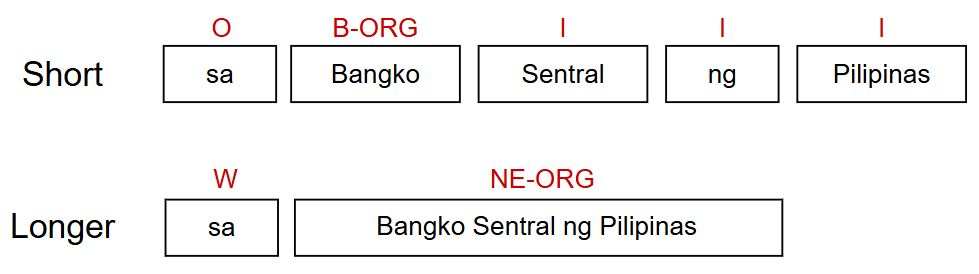
\includegraphics[scale=0.43]{images/IOB Tagging and Labelling - Close Up.JPG}
    \captionsetup{justification=centering}
    \caption{An example of short and longer unit tokenization with labels. In short unit tokenization, tokens are labeled using IOB tagging. In contrast, for longer unit tokenization, the Tagalog NEs and multi-word expressions are labeled based on PANG-KAT's dictionary categories, while other tokens are labeled as "W".
}
\end{figure}

\begin{table}[H]
    \centering % instead of \begin{center}
    \captionsetup{justification=centering}
    \caption{PANG-KAT labels for short and longer unit tokenization, with their descriptions.}  \label{tab:effects}
    \vspace{1mm} % Adjust the height of the space between caption and tabular

    \renewcommand{\arraystretch}{1.5}
    \fontsize{12pt}{12pt}\selectfont
    \resizebox{\columnwidth}{!}{%
\begin{tabular}{|c|c|c|}
\hline
\textbf{CATEGORY}                         & \textbf{LABELS} & \textbf{DESCRIPTION}                                                          \\ \hline
\multirow{Short Unit Tokenization}  & B-ORG           & Beginning of organization NEs                                                 \\ \cline{2-3} 
                                          & B-LOC           & Beginning of location NEs                                                     \\ \cline{2-3} 
                                          & B-PER           & Beginning of person NEs                                                       \\ \cline{2-3} 
                                          & B-MWE           & Beginning of MWEs                                                             \\ \cline{2-3} 
                                          & I               & Inside/part of NEs or MWEs                                                    \\ \cline{2-3} 
                                          & O               & \begin{tabular}[c]{@{}c@{}}Outside/not part of any \\ NE or MWE\end{tabular}  \\ \hline
\multirow{Longer Unit Tokenization} & NE-ORG          & Organization named entity                                                     \\ \cline{2-3} 
                                          & NE-LOC          & Location named entity                                                         \\ \cline{2-3} 
                                          & NE-PER          & Person named entity                                                           \\ \cline{2-3} 
                                          & MWE             & Multi-word expression                                                         \\ \cline{2-3} 
                                          & W               & \begin{tabular}[c]{@{}c@{}}Not a NE or MWE, \\ an ordinary word.\end{tabular} \\ \hline
    \end{tabular} %
    }
\end{table}

\subsection {Performance Evaluation}

The author, in collaboration with two native Tagalog speaker annotators, will annotate the sentences from the testing set of the NewsPH-NLI Dataset {\cite{NewsPH-NLI}} for both short and longer unit tokenization. This dataset contains data retrieved from published news articles in the Philippines, which mostly exhibit instances of Tagalog NEs, MWEs, and Tagalog-English code-switching. Additionally, latest and complete articles from Pilipino Star Ngayon {\cite{PhilStar}} as of May 2025 will also be annotated to evaluate PANG-KAT's adaptability to recent Tagalog language resources and full-length news texts. \\

The performance of PANG-KAT tokenization capabilities will be evaluated on the annotated sentences of the NewsPH-NLI Dataset and the annotated articles of Pilipino Star Ngayon using the following performance evaluation metrics:\\

\begin{itemize}
  \item \textbf{Accuracy:} This performance metric quantifies how the algorithm groups the data points accurately  {\cite{perEvalMetrics}} \\

    \begin{center}
    \fontsize{12pt}{12pt}\selectfont
    Accuracy = \(\frac{TP + TN}{TP + TN + FP + FN }\)
    \end{center} \bigskip
  
  \item \textbf{Precision:} This performance metric refers to the portion of true positives out of all significant instances  {\cite{perEvalMetrics}} \\

    \begin{center}
    \fontsize{12pt}{12pt}\selectfont
    Precision = \(\frac{TP}{TP + FP}\)
    \end{center} \bigskip

  \item \textbf{Recall or Sensitivity:} This performance metric refers to the portion of true positives among all applicable instances  {\cite{perEvalMetrics}} \\

    \begin{center}
    \fontsize{12pt}{12pt}\selectfont
    Recall = \(\frac{TP}{TP + FN}\)
    \end{center} \bigskip

  \item \textbf{F1 Score:} This performance metric refers to the harmonic mean of the recall and precision. The higher the F1 score, the closer the precision and recall  {\cite{perEvalMetrics}}\\

  \begin{center}
  \fontsize{12pt}{12pt}\selectfont
  F1 Score = 2 * \(\frac{Precision * Recall}{Precision + Recall}\)
  \end{center} \bigskip

\end{itemize}

% RESULTS AND DISCUSSION
\section{Results and Discussion}


\subsection {Graphical User Interface (GUI) Development}

PANG-KAT was design to be implemented as a Python module, which can be imported into more advanced Tagalog NLP applications as its tokenizer. To facilitate the evaluation of its performance, a GUI was developed to provide a visual representation of its tokenization results. In the module, these results of PANG-KAT are returned in arrays of tokens and their corresponding labels for both short and longer unit tokenization. The GUI of PANG-KAT is developed using Tkinter, which is the standard Python library for graphical interfaces and serves as an interface to the Tcl/Tk GUI toolkit that provides a comprehensive library for building GUIs {\cite{Python3}}. The font and image used as assets in the development of the GUI were retrieved and imported from publicly available external sources. \\

\subsubsection{Welcome Screen}

PANG-KAT's welcome screen was straightforward. Upon clicking the start button, the user will be redirected to the file selection screen. Otherwise, clicking the exit button will close PANG-KAT.

\begin{figure}[H]
    \centering
    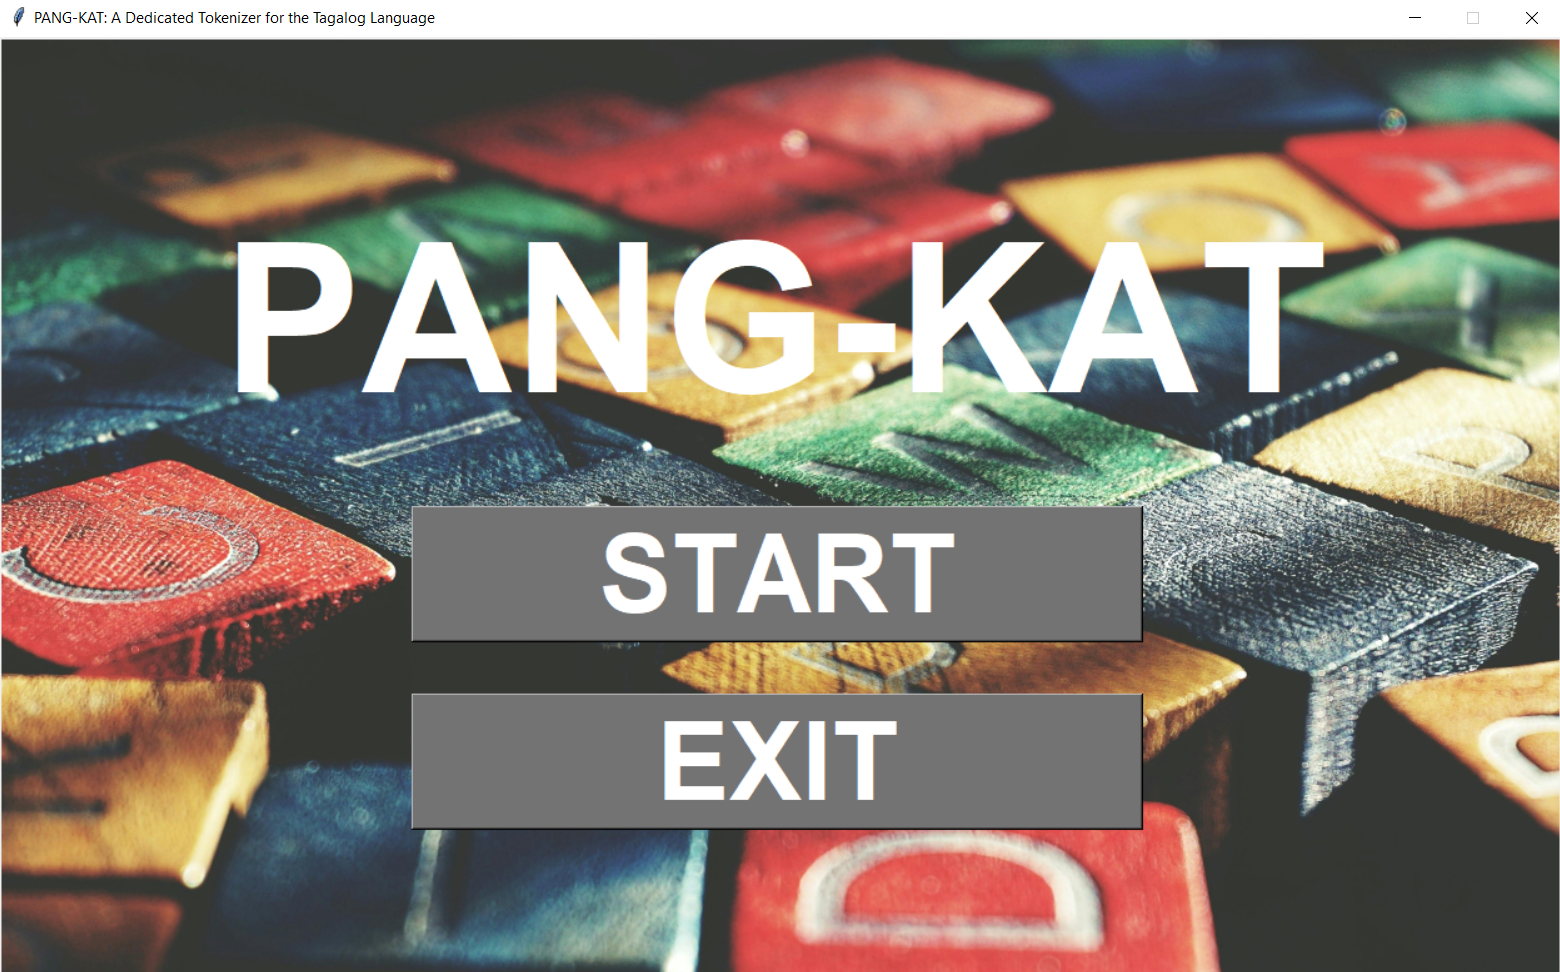
\includegraphics[scale=0.27]{images/Welcome Screen.png}
    \captionsetup{justification=centering}
    \caption{The Welcome Screen of PANG-KAT}
\end{figure}

\subsubsection{File Selection Screen}

In the file selection screen, a button for choosing the file containing the data the user wants to be tokenized can be seen. Upon clicking this button, a file dialog window will be opened to allow the user to locate and choose this file.

\begin{figure}[H]
    \centering
    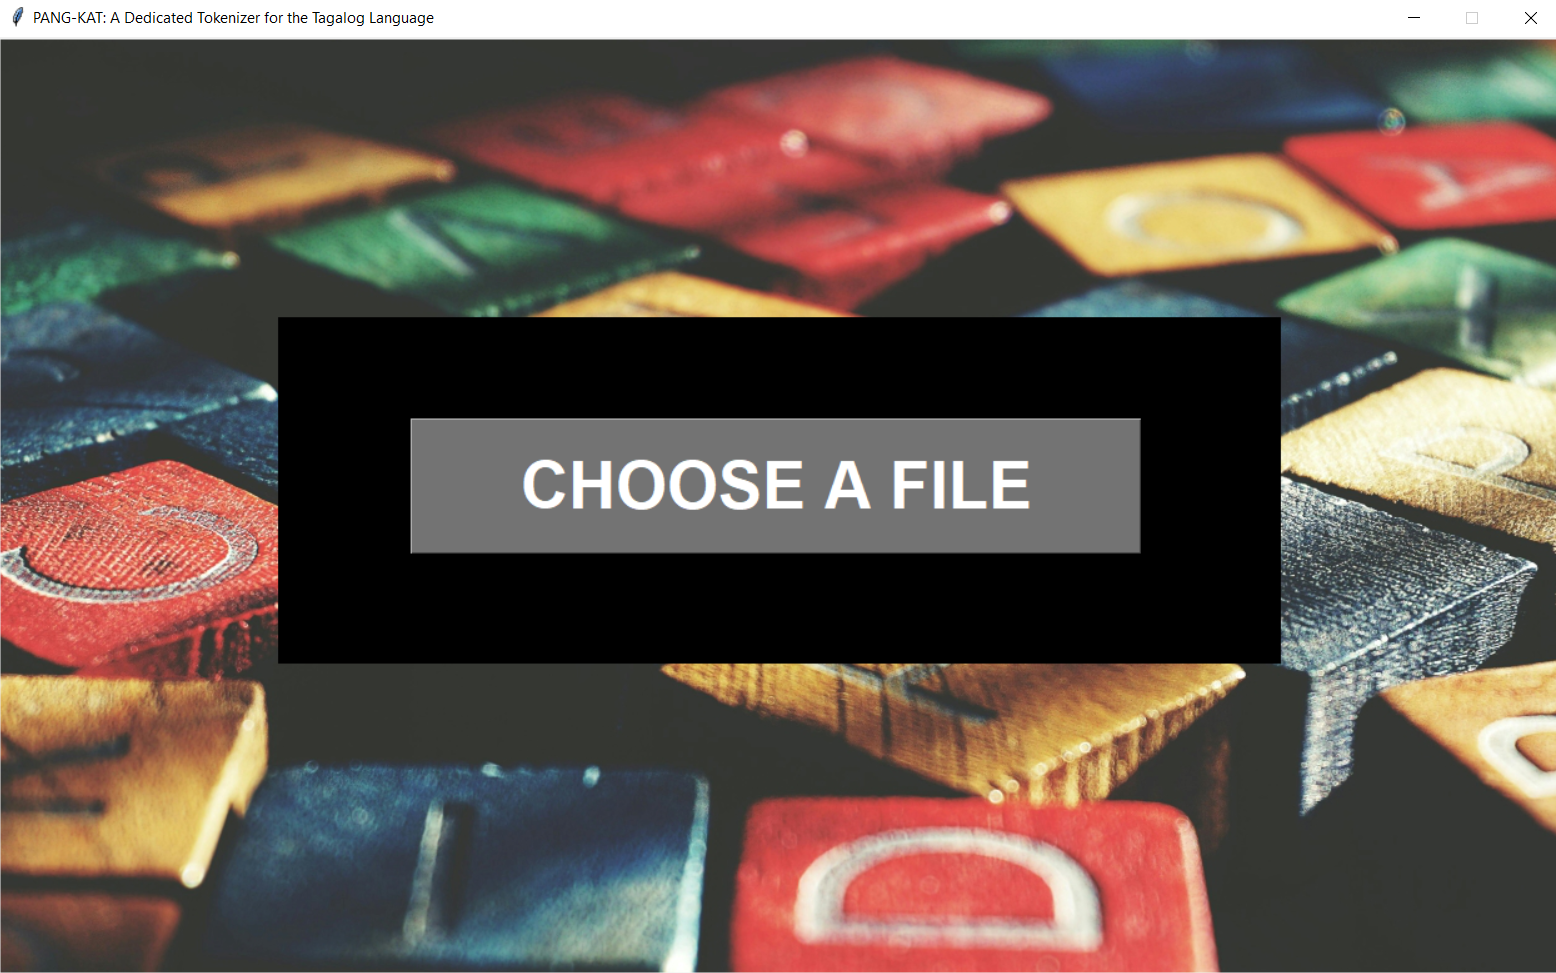
\includegraphics[scale=0.27]{images/File Selection Screen 1.png}
\end{figure}

\begin{figure}[H]
    \centering
    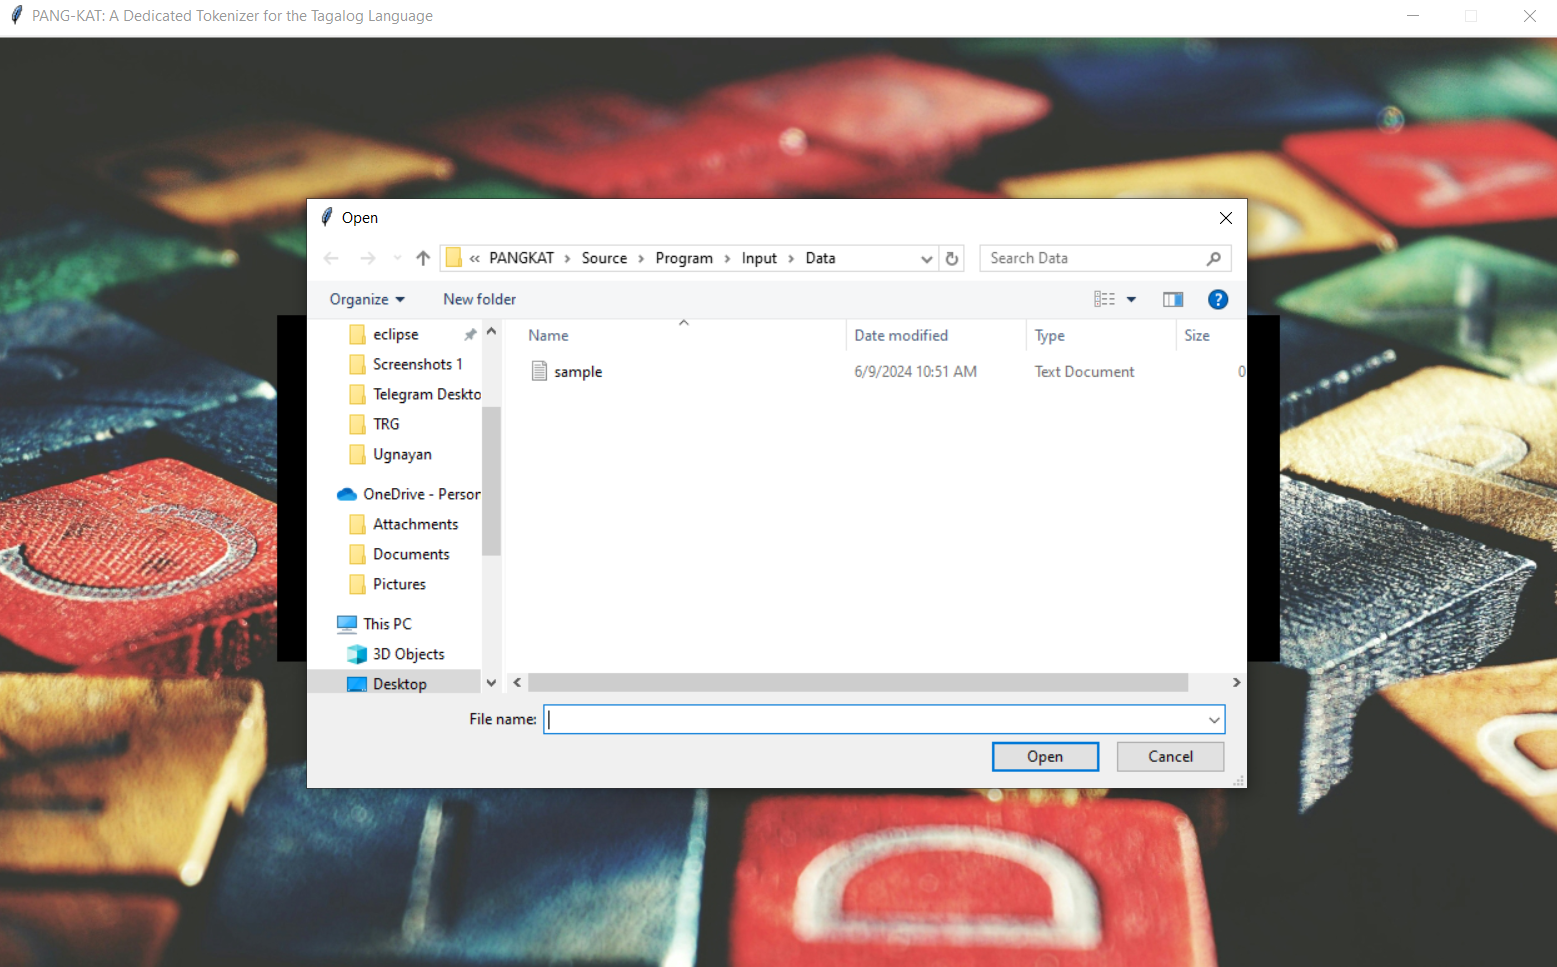
\includegraphics[scale=0.27]{images/File Selection Screen 2.png}
    \captionsetup{justification=centering}
    \caption{The File Selection Screen of PANG-KAT.}
\end{figure}

\begin{figure*}[]
    \centering
    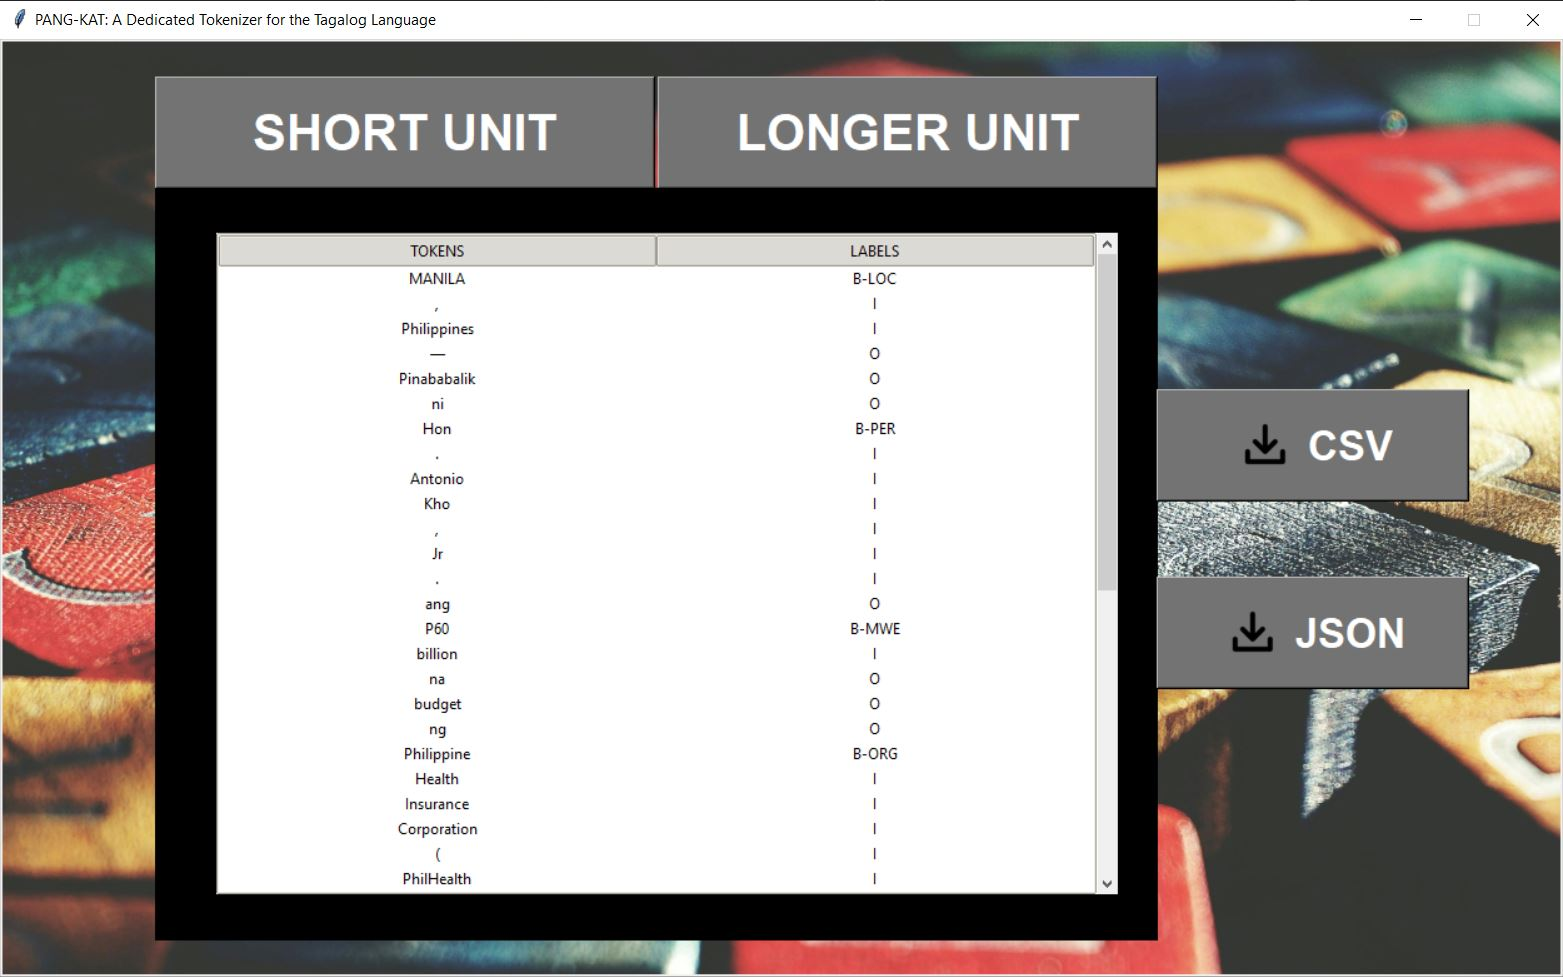
\includegraphics[scale=0.5]{images/Short Unit Tokenization - Demo.JPG}
    \captionsetup{justification=centering}
    \caption{The Results Screen of PANG-KAT for short-unit tokenization. }
\end{figure*}

\begin{figure*}[]
    \centering
    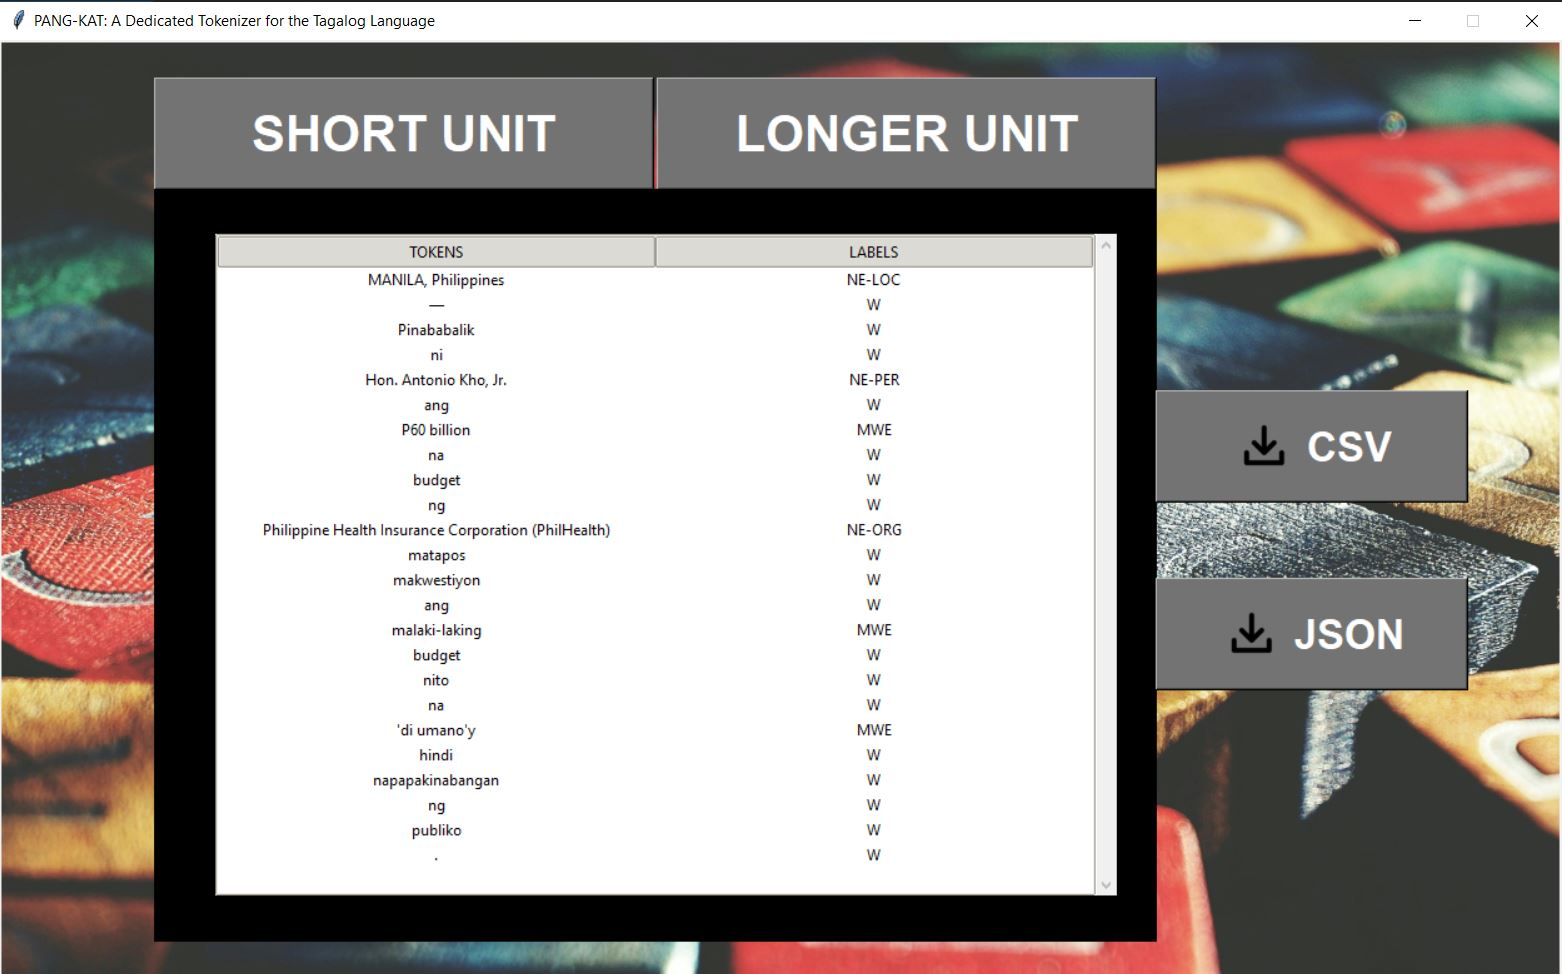
\includegraphics[scale=0.5]{images/Longer Unit Tokenization - Demo.JPG}
    \captionsetup{justification=centering}
    \caption{The Results Screen of PANG-KAT for longer-unit tokenization.}
\end{figure*}

\newpage

\subsubsection{Results Screen}

In the results screen, a table presenting the resulting tokens and their corresponding labels can be seen. Above the table are two buttons for toggling the results shown in the table between short and longer unit tokenization. To the right side of the table are buttons for downloading the results in either CSV or JSON format. \\ 

\subsection {Results}

\subsubsection{Dictionary Creation}

The dictionary for PANG-KAT was created by extracting Tagalog named entities (NEs) from the TLUnified-NER corpus, multi-word expressions (MWEs) from an online Tagalog dictionary using a Tagalog Dictionary Scraper, and manually sourcing additional data from various online resources for each specific type of NE. \\

\begin{table}[H]
    \centering % instead of \begin{center}
    \captionsetup{justification=centering}
    \caption{The dictionary size and composition of PANG-KAT.}  \label{tab:effects}
    \vspace{1mm} % Adjust the height of the space between caption and tabular

    \renewcommand{\arraystretch}{1.5}
    \fontsize{12pt}{12pt}\selectfont
    \resizebox{\columnwidth}{!}{%

    \begin{tabular}{|c|c|}
    \hline
    \textbf{CATEGORY}                         & \textbf{TOKEN COUNT} \\ \hline
    Location entities (NE-LOC)                & 48,383               \\ \hline
    Organization entities (NE-ORG)            & 3,564                \\ \hline
    Person Entities (NE-PER)                  & 7,321                \\ \hline
    Multi-word Expressions (MWE)              & 3,294                \\ \hline
    \textbf{PANG-KAT’s Total Dictionary Size} & \textbf{62,562}      \\ \hline
    \end{tabular} %
    }
\end{table}

For location entities, additional entities are gathered from an online Philippine Atlas, which contains information regarding the list of all regions, provinces, municipalities, cities, and barangays in the Philippines {\cite{PhilAtlas}}. Combined with location entities extracted from the TLUnified-NER, a total of 48,383 location entities were sourced for inclusion in PANG-KAT's dictionary. \\

Moreover, additional organization entities were gathered from the Department of Budget and Management’s {\cite{DBM-OCIO}}{\cite{OrgAcronyms}} list of national government offices, agencies, bureaus, government-owned and controlled corporations, and their respective abbreviations. The list of accredited non-government and non-profit organizations in the Philippines was also extracted and added from the Philippine Council for NGO Certification {\cite{NGO}}. Combined with the organization entities extracted from the TLUnified-NER, a total of 3,564 organization entities were sourced for inclusion in PANG-KAT’s dictionary. \\

Furthermore, additional person entities were gathered from various publicly available datasets containing a list of the most common Filipino names {\cite{nameDatabase}} {\cite{popNameDatabase}}, and famous Filipino celebrities {\cite{filCelebs}}. Data regarding renowned Filipino politicians and their positions was also included {\cite{worldLeaders}} {\cite{Senators}}. Combined with the person entities extracted from the TLUnified-NER, a total of 7,321 person entities were sourced for inclusion in PANG-KAT’s dictionary. \\

Lastly, additional Tagalog MWEs were gathered from resources with support for MWEs {\cite{KWFManwal}}, which, when combined with the Tagalog MWEs extracted from the Tagalog Dictionary scraper, yielded a total of 3,294 MWEs for inclusion in PANG-KAT’s dictionary. Therefore, the total dictionary size of PANG-KAT is composed of 62,562 Tagalog NEs and MWEs, which are categorized into Person entities (NE-PER), Organization entities (NE-ORG), Location entities (NE-LOC), and multi-word expressions (MWE). The researcher’s effort in expanding PANG-KAT’s dictionary is crucial for improving the overall performance of PANG-KAT in detecting and classifying Tagalog NEs and MWEs. \\

\subsubsection{TweetTaglish Annotation}

The author, in collaboration with two native Tagalog speaker annotators, was able to annotate the TweetTaglish corpus using Inside–Outside–Beginning (IOB) tagging. The resulting annotated corpus is composed of 1,858 sentences with 34,424 labeled tokens, which will be used in observing patterns in Tagalog and English (Taglish) code-switching that will be incorporated in the rule extraction phase to make PANG-KAT capable of Taglish tokenization. \\

\begin{table}[H]
    \centering % instead of \begin{center}
    \captionsetup{justification=centering}
    \caption{The composition of the annotated TweetTaglish Corpus.}  \label{tab:effects}
    \vspace{1mm} % Adjust the height of the space between caption and tabular

    \renewcommand{\arraystretch}{1.5}
    \fontsize{11pt}{11pt}\selectfont
    \begin{tabular}{|c|c|}
    \hline
    \textbf{LEGEND} & \textbf{COUNT} \\ \hline
    Sentences       & 1858           \\ \hline
    Labeled Tokens  & 34,424         \\ \hline
    \end{tabular}
\end{table}

\subsubsection{Rules Extraction}

The rules of PANG-KAT are manually extracted from the Tagalog Reference Grammar (TRG) {\cite{TRG}} and Ugnayan {\cite{Ugnayan}} treebanks, which are to be used in detecting Tagalog named entities (NEs) and multi-word expressions (MWEs) that follow a certain format. To better capture Tagalog language patterns, these initial rules are cross-referenced with the Komisyon sa Wikang Filipino (KWF) Manwal sa Masinop na Pagsulat {\cite{KWFManwal}}, from which additional rules were also extracted. Afterward, the rules were tested on the annotated TweetTaglish corpus to adapt the rules for Tagalog and English (Taglish) code-switching. The following subsections present these rules and their corresponding descriptions. \\

\paragraph{Intensification}

The meaning of Tagalog adjectives and pseudo-verbs can be intensified using the connectors “na” or “-ng”. Tagalog pseudo-verbs are words that are not classified as verbs but function similarly, commonly used to express desire, necessity, ability, or obligation before an action. Tagalog Pseudo-verbs includes "ayaw", "gusto", "kaya", "pwede", "kailangan", and "dapat" {\cite{LearningTagalog}}. Similarly, the meaning of Tagalog verbs and adverbs can also be intensified using the conjunction “at”. \\ \\

Examples:

\begin{multicols}{2}
    \begin{itemize}
      \item malungkot \textbf{na} malungkot \\
    
      \item ayaw \textbf{na} ayaw \\

      \item darating \textbf{at} darating\\
    
      \item maganda\textbf{ng} maganda \\
    
      \item gusto\textbf{ng} gusto\\
    
      \item lagi \textbf{at} laging \\
    \end{itemize}
\end{multicols}

\paragraph{Continuity of Action}

Tagalog verbs and adverbs can be connected with the conjunction “nang” to signify a continuous progression of a particular action. \\

Examples: \\

\begin{itemize}
  \item tumakbo \textbf{nang} tumakbo \\

  \item palakas \textbf{nang} palakas \\
\end{itemize}

\paragraph{Repeating words}

Tagalog nouns, verbs, adjectives, and adverbs can be repeated to introduce variation in their meaning. This repetition of words can be plain, partial reduplication, with the addition of prefixes, infixes, or the "ang" marker to add more focus to the description of the repeating word. Tagalog repeating words are traditionally written with a hyphen. However, it is acceptable and not uncommon for traditionally hyphenated repeating words to be still written without a hyphen, particularly in colloquial writing. \\

Examples: \\


    \begin{itemize}
      \item gaya-gaya / gaya gaya \\
      \item kani-kanila / kani kanila \\
      \item nagtuloy-tuloy / nagtuloy tuloy \\
      \item tinali-tali / tinali tali \\
      \item tumalon-talon / tumalon talon \\
      \item ang lungkot-lungkot / ang lungkot lungkot \\
    \end{itemize}
    
\paragraph{Contractions}

In Tagalog colloquial writing, it is common to contract the “ay” marker and the “at” conjunction to make it more fluid and natural. Contraction also happens in cases of "kambal-patinig", which occurs when two consecutive vowel sounds appear in a word and lead to the omission of the first vowel sound {\cite{KWFManwal}}. Kambal-patinig often appears at the first syllable of a word that starts with a consonant letter, but can also appear at the start of a word. Additionally, years can also be contracted in writing, and some Tagalog words that are traditionally contracted in common speech also appear in their contracted form when written. \\ \\

Examples:

\begin{multicols}{2}
    \begin{itemize}
      \item ako ay $\rightarrow$ ako‘y \\
      \item dalawampu at apat $\rightarrow$ dalawampu’t apat  \\
      \item siya $\rightarrow$ s’ya \\
      \item iyan $\rightarrow$ ‘yan \\
      \item 1997 $\rightarrow$ ‘97 \\
      \item huwag $\rightarrow$ ‘wag \\
    \end{itemize}
\end{multicols}

\paragraph{Date and Time}

In Tagalog, the prefix “ika-” is used in both date and time expressions. For dates, "ika-" indicates the specific day of the month, following the format: "ika-\# ng [buwan]" (e.g., ika-15 ng Abril for April 15). An informal way to express dates in Tagalog uses the prefix "a-" combined with borrowed Spanish numbers, following the format: "a-[Spanish-number] ng [buwan]" (e.g., a-kinse ng Abril for April 15). However, this format is more commonly used in everyday speech than writing. For time, “ika-” indicates the specific hour of the day, following the format: “ika-[Tagalog-number] ng [Tagalog-time-indicator]” (e.g., ika-tatlo ng hapon for 3 PM). Tagalog time indicators include  “umaga”, “tanghali”, “hapon”, “dapithapon”, “gabi”, “hatinggabi” at “madaling araw”. \\ 

Spanish influence also exists in the informal way of expressing time in Tagalog, which uses the Spanish word “ala/alas” combined with borrowed Spanish numbers, following the format: “ala/alas [Spanish-number] ng [Tagalog-time-indicator]” (e.g., alas tres ng hapon for 3 PM). This format is more commonly used in both speech and writing compared to the "ika-" format. \\

Aside from these formats, it is also common in Taglish code-switching to express date using the following English formats: Month-Day-Year (e.g., April 15, 2025, Apr. 15, 2025, 04-15-2025, 04/15/2025), Day-Month-Year (e.g., 15 April 2025, 15 APR 2025, 15-04-2025, 15/04/2025), and Year-Month-Day (e.g., 2025/04/25, 2025-04-25) that aligns with the ISO 8601 standard {\cite{ISO8601}}. For time formats, the English 12-hour clock system (e.g. 03:00 p.m., 03:00 PM, 3 PM) and the 24-hour clock system (e.g. 15:00 for 3 PM) were also commonly used in Taglish code-switching. \\

\paragraph{Borrowed Spanish Conjunction “y”}

In connection with the Spanish influence on how time is expressed in Tagalog, the Spanish conjunction "y", which translates to "and" in English, has also been incorporated when expressing specific times in Tagalog. For instance, in Tagalog, 3:30 PM can be expressed as "alas tres y medya ng hapon". Spanish numbers, which use "y" to express digits above 30, are used for expressing more specific times (e.g., alas tres y treynta y dos ng hapon for 3:32 PM). Additionally, “impunto” is used to indicate the exact hour (e.g., alas tres impunto ng hapon for 3:00 PM), and “pasado” to indicate that a specific time had already passed (e.g., pasado alas tres ng hapon for past 3 PM). \\

Aside from time expressions, Spanish numbers below 100 remain commonly used in Tagalog, though they are more common in speech than writing. Lastly, during the Spanish colonial period, "y" was used to connect a person's maternal surname to their full name (e.g., Jose Protasio Rizal Mercado y Alonso Realonda). However, this format has long faded in modern times and is now mostly found in the names of Filipino historical figures. \\

\paragraph{Daglat}

Daglat refers to the abbreviation of words and expressions in the Tagalog language. It is commonly used for Tagalog titles, honorifics, and the names of Filipino organizations and government institutions. Additionally, certain Tagalog time indicators have their accepted abbreviations, such as n.u. ng umaga), n.h. (ng hapon), and n.g. (ng gabi). However, these are rarely used today and are largely replaced by their more common English equivalents, "a.m." and "p.m.". \\

Most abbreviations end with a period, such as Tagalog titles and honorifics before a person’s name (e.g., Engr. Pangilinan, Mr. Pangilinan). However, titles placed after a person's name may be written with or without a period, with the modern trend favoring the omission of periods and separated by a comma from the person’s name (e.g., Pangilinan, PhD). Similarly, the daglat for organizations and government institutions is generally written without periods (e.g., DepEd). \\

\paragraph{Spelled-Out Tagalog Large Numbers}

Tagalog numbers utilize numerical classifiers like "daan", "libo", “"daang libo", “daang milyon”, “daang milyon” and “daang trilyon” to express hundreds, thousands, hundred thousand, hundred million, hundred billion, and hundred trillion, respectively. In formal writing, numbers that precede these numerical classifiers should be spelled out (e.g., limampu’t isang libo, walong daang libo). However, for the numerical classifiers "milyon", “bilyon”, and "trilyon", which correspond to million, billion, and trillion, numbers from 1 to 10 that precede these classifiers should be spelled out (e.g., sampung milyon), while larger numbers are written in numerical form (e.g., 12 bilyon) {\cite{KWFManwal}}. This same rule applies to their equivalent English numerical classifiers. In Taglish and colloquial writing, large numbers are more commonly written in their numerical form, arranged in groups of three digits from right to left, and separated by commas or spaces (e.g., 5,000 or 5 000). \\

\paragraph{Beginning Markers}

During the annotation process of the TweetTaglish corpus, Tagalog prefixes have been observed as common beginning markers for Taglish code-switching. This indicates that when the two languages are mixed, the most frequently observed pattern is the addition of Tagalog prefixes to English words. Similar to Tagalog constructions, Tagalog prefixes may be added to English nouns, verbs, adjectives, and adverbs. In formal writing, the combination of a Tagalog prefix + English word commonly includes the use of a hyphen as a morphological boundary (e.g., nakaka-stress). However, hyphens are often omitted in colloquial writing, which results in combinations that are either concatenated (e.g., nakakastress) or separated by a space (e.g., nakaka stress), as consistently observed in the TweetTaglish corpus. In addition to prefixes, the Tagalog plural marker "mga" was also observed as a common beginning marker to indicate plurality in both Tagalog and English words. \\

The list of identified beginning markers includes:\\

\begin{multicols}{3}
    \begin{itemize}
      \item "mga" \\
      \item "mag" \\
      \item "magka" \\
      \item "magpa" \\
      \item "magkaka" \\
      \item "magpapa" \\
      \item "maka" \\
      \item "makaka" \\
      \item "makapag" \\
      \item "makakapag" \\
      \item "mapag" \\ 
      \item "nag" \\
      \item "nagka" \\
      \item "nagpa" \\
      \item "nagkaka" \\
      \item "nagpapa" \\
      \item "naka" \\
      \item "napapa" \\
      \item "nakaka" \\
      \item "nakapag" \\
      \item "nakakapag" \\
      \item "napaka" \\
      \item "napag" \\
      \item "pag" \\
      \item "pagka" \\
      \item "pagpa" \\
      \item "pagkaka" \\
      \item "pagpapa" \\
      \item "paka" \\
      \item "papapa" \\
      \item "pakaka" \\
      \item "pina" \\
      \item "pinag" \\
      \item "ipa" \\
      \item "ipinag" \\
      \item "ipinagka" \\
      \item "ipinagpa" \\
      \item "ipinagkaka" \\
      \item "ipinagpapa" \\
      
    \end{itemize}
\end{multicols}

Examples:

\begin{itemize}
  \item mag + ma + marites = magma-marites / magmamarites / magma marites \\
  \item ipa + consult = ipa-consult / ipaconsult / ipa consult \\
  \item pagka + bitter = pagka-bitter / pagkabitter / pagka bitter \\
  \item napaka + close = napaka-close / napakaclose / napaka close \\
\end{itemize}

\paragraph{Punctuation and Other Symbols}

Most of the previously discussed language rules frequently employed the use of various punctuation. This section provides a table summarizing the identifiable uses of these punctuations and other symbols that are identifiable by PANG-KAT. \\ \\ 

\begin{table*}[]
\centering % instead of \begin{center}
\captionsetup{justification=centering}
\caption{Punctuations, other symbols, and their recognizable uses by PANG-KAT.}  \label{tab:effects}
\vspace{1mm} % Adjust the height of the space between caption and tabular
\renewcommand{\arraystretch}{1.5}
\fontsize{11pt}{11pt}\selectfont
\begin{tabular}{|c|c|}
\hline
\textbf{\begin{tabular}[c]{@{}c@{}}PUNCTUATION\\ AND OTHER SYMBOLS\end{tabular}}                                                             & \textbf{USES}                                                                                                                                                                                                                                                                                                                                                                                                                                                                               \\ \hline
Apostrophe (’)                                                                    & \begin{tabular}[c]{@{}c@{}}For signifying the contraction of \\ words or years.\end{tabular}                                                                                                                                                                                                                                                                                                                                                                                                \\ \hline
Hyphen (-)                                                                        & \begin{tabular}[c]{@{}c@{}}For connecting repeating words, \\ one-syllable onomatopoeic sounds (e.g., ding-dong), \\ and tambalans (e.g., lipat-bahay).\\ \\ For separating consecutive syllables where the preceding one ends \\ with a consonant and the succeeding one starts with a vowel (e.g., pag-asa) \\ and phone numbers (e.g., 0987-654-3210).\\ \\ In writing date, time, and a word letter by letter \\ or based on how it is pronounced (e.g.,  PAG-BA-BAY-BAY).\end{tabular} \\ \hline
Period (.)                                                                        & \begin{tabular}[c]{@{}c@{}}For writing decimal numbers (e.g., 1.91) and \\ it is placed at the end of daglat.\end{tabular}                                                                                                                                                                                                                                                                                                                                                                  \\ \hline
Colon (:)                                                                         & For writing the English time format (e.g., 9:30 AM).                                                                                                                                                                                                                                                                                                                                                                                                                                        \\ \hline
Comma (,)                                                                         & \begin{tabular}[c]{@{}c@{}}For separating numbers (e.g., 1,000) and \\ titles placed at the end of a person’s name.\\ \\ For writing names in \textless{}Surname\textgreater{}, \textless{}Name\textgreater format, \\ and in English date format (e.g., April 15, 2025).\end{tabular}                                                                                                                                                                                                      \\ \hline
Slash (/)                                                                         & \begin{tabular}[c]{@{}c@{}}For writing English date format(e.g., 04/15/2025) and \\ indicating choices (e.g., abogado/a).\end{tabular}                                                                                                                                                                                                                                                                                                                                                   \\ \hline
\begin{tabular}[c]{@{}c@{}}Parenthesis (()), Brackets ({[}{]}), \\ and Braces (\{\})\end{tabular} & \begin{tabular}[c]{@{}c@{}}For specifying known abbreviations of \\ some named entities (e.g., Department of Health (DOH) or {[}DOH{]}).\end{tabular}                                                                                                                                                                                                                                                                                                                                       \\ \hline
Basic Mathematical Symbols                                                                        & \begin{tabular}[c]{@{}c@{}}This includes addition (+), subtraction (-), multiplication (x), division (/), \\ exponentiation (\textasciicircum{}), percentage (\%), degrees (°), Euler's number (e),  \\ natural logarithm (ln), logarithm (log), and square root (sqrt or $\sqrt{}$).\end{tabular}

            \\ \hline

\end{tabular}
\end{table*}

\newpage

\paragraph{Rules sequencing}

The sequence of PANG-KAT rules prioritizes rules with more structured, language-specific patterns over more general rules and dictionary lookups. These include rules with specific formats that utilize distinct Tagalog markers, such as: \\ 

\begin{itemize}
    \item MWEs that start with beginning markers. \\
    \item Tagalog date and time expressions that utilize "ika-", "a-", and "ala/alas". \\
    \item Uses of the borrowed Spanish conjunction “y”. \\
    \item Spelled-Out Tagalog Large Numbers with their Tagalog numerical classifiers. \\
    \item Intensification and continuity of actions that utilize “na”, “-ng”, “at”, and “nang”. \\
    \item Structured repeating word patterns, which may also utilize Tagalog prefixes, infixes, and the “ang” marker. \\
\end{itemize}

These rules are prioritized due to their highly structured and predictable nature, which ensures a high degree of accuracy when matched. This behavior is due to these rules being tailored to capture the unique morphological and syntactic patterns of the Tagalog language, which are not easily generalized across languages. By processing these first, PANG-KAT is able to accurately identify and label multi-word expressions that span multiple tokens. Thus, minimizing the risk of possible mislabeling caused by broader, more general rules. \\

Following these structured, language-specific patterns are more general rules that include the various uses of different punctuations and numerical formats, which are not specific to the Tagalog language and are more prone to ambiguity. When a punctuation mark has a language-specific use, this specific function must take precedence within its corresponding rule block. For instance, the contracted “at” in phrases like “dalawampu’t isa” should be prioritized due to its specific use that connects the two words together. These rules are highly dependent on their immediate neighbors. Thus, they are placed before the broadest layer of processing, which is the dictionary-based lookups that are executed last. \\

Dictionary-based lookups are applied only after all syntactic and morphological patterns have been evaluated. This is because they are prone to overgeneralization that could mislabel language-specific patterns. For instance, if dictionary lookup comes first when labeling “alas dos ng umaga”, it could mislabel “alas” as a possible name of a person. Thus, tokenizing a coherent time expression incorrectly, which would result in the erasure of its temporal meaning. This highlights the importance of PANG-KAT’s rule sequencing, which preserves language-specific structures by prioritizing the matching of their more structured, language-specific patterns in the pipeline. \\

PANG-KAT operates on a linear, first-match-wins architecture, wherein when a token is labeled, it won’t be reconsidered by later rules. Thus, its rule sequencing is crucial for ensuring accurate token-labelling. Token labels are only updated based on specific triggers. For instance, in the phrase “Pasig Mayor Vico Sotto,” the token Pasig would be initially labelled as a location (B-LOC), but would be updated as part of a person entity (B-PER) after matching the full entity using the B-PER dictionary. Through this architecture, overgeneralization caused by general rules is resolved by handling more structured, language-specific patterns first. \\

\paragraph{Unit Testing}

All previously discussed language rules were converted into code and integrated into the rule set of PANG-KAT, combined with the algorithm that utilizes the discussed dictionaries for detecting named entities and multi-word expressions. To ensure that these rules are functioning correctly, unit testing was conducted using the TRG, Ugnayan, and annotated TweetTaglish corpus for both short and longer unit tokenization. The output of PANG-KAT on these datasets was evaluated on each of their true labels, which yielded F1 scores of 0.9735, 1.0, and 0.9713 for short unit tokenization and 0.9735, 1.0, and 0.9709 for longer unit tokenization, respectively. Given that the F1 score ranges from 0 to 1 {\cite{perEvalMetrics}}, the following F1 scores for PANG-KAT’s unit testing indicate that it was able to almost perfectly tokenize and classify Tagalog NEs and MWEs for both short and longer unit tokenization. \\

\begin{table}[H]
    \centering % instead of \begin{center}
    \captionsetup{justification=centering}
    \caption{The composition of the datasets used for PANG-KAT’s unit testing.}  \label{tab:effects}
    \vspace{1mm} % Adjust the height of the space between caption and tabular
    \renewcommand{\arraystretch}{1.5}
    \fontsize{11pt}{11pt}\selectfont        \resizebox{\columnwidth}{!}{%

    \begin{tabular}{|c|c|c|}
    \hline
    \textbf{DATASET} & \textbf{SENTENCES} & \textbf{\begin{tabular}[c]{@{}c@{}}LABELLED TOKENS\end{tabular}} \\ \hline
    TRG              & 128                & 734                                                                 \\ \hline
    Ugnayan          & 94                 & 1,025                                                               \\ \hline
    TweetTaglish     & 1,858               & 34,424                                                              \\ \hline
    \end{tabular}%
    }
\end{table}

\begin{table}[H]
    \centering % instead of \begin{center}
    \captionsetup{justification=centering}
    \caption{Unit testing results for PANG-KAT’s short-unit tokenization.}  \label{tab:effects}
    \vspace{1mm} % Adjust the height of the space between caption and tabular
    \renewcommand{\arraystretch}{1.5}
    \fontsize{102pt}{200pt}\selectfont
    \resizebox{\columnwidth}{!}{%

    \begin{tabular}{|c|c|c|c|c|}
    \hline
    \textbf{DATASETS} & \textbf{ACCURACY} & \textbf{PRECISION} & \textbf{RECALL} & \textbf{F1-SCORE} \\ \hline
    TRG               & 0.9959            & 0.9649             & 0.9821          & 0.9735            \\ \hline
    Ugnayan           & 1.0               & 1.0                & 1.0             & 1.0               \\ \hline
    TweetTaglish      & 0.9943            & 0.9753             & 0.9981          & 0.9865            \\ \hline
    \end{tabular} %
    }
\end{table}

\begin{table}[H]
    \centering % instead of \begin{center}
    \captionsetup{justification=centering}
    \caption{Unit testing results for PANG-KAT’s longer-unit tokenization.}  \label{tab:effects}
    \vspace{1mm} % Adjust the height of the space between caption and tabular
    \renewcommand{\arraystretch}{1.5}
    \fontsize{102pt}{200pt}\selectfont
    \resizebox{\columnwidth}{!}{%

    \begin{tabular}{|c|c|c|c|c|}
    \hline
    \textbf{DATASETS} & \textbf{ACCURACY} & \textbf{PRECISION} & \textbf{RECALL} & \textbf{F1-SCORE} \\ \hline
    TRG               & 0.9958            & 0.9473             & 0.9730          & 0.9600            \\ \hline
    Ugnayan           & 1.0               & 1.0                & 1.0             & 1.0               \\ \hline
    TweetTaglish      & 0.9931            & 0.9443             & 0.9968          & 0.9698            \\ \hline
    \end{tabular}%
    }
\end{table}

\subsubsection{Performance Evaluation}

 The author, in collaboration with two native Tagalog speaker annotators, was able to annotate the NewsPH-NLI Dataset using Inside–Outside–Beginning (IOB) tagging. The resulting annotated dataset is composed of 881 sentences with 28.922 labeled tokens, which served as the true labels in validating the output of PANG-KAT on this dataset to evaluate its performance for both short and longer unit tokenization. The performance evaluation results yielded F1 scores of 0.9518 and 0.9130 for short and longer unit tokenization, respectively. \\

\begin{table}[H]
    \centering % instead of \begin{center}
    \captionsetup{justification=centering}
    \caption{The composition of the annotated NewsPH-NLI Dataset.}  \label{tab:effects}
    \vspace{1mm} % Adjust the height of the space between caption and tabular
    \renewcommand{\arraystretch}{1.5}
    \fontsize{11pt}{11pt}\selectfont

    \begin{tabular}{|c|c|}
    \hline
    \textbf{LEGEND} & \textbf{COUNT} \\ \hline
    Sentences       & 881            \\ \hline
    Labeled Tokens  & 28,922         \\ \hline
    \end{tabular}
\end{table}

\begin{table}[H]
    \centering % instead of \begin{center}
    \captionsetup{justification=centering}
    \caption{Performance evaluation results of PANG-KAT on the NewsPH-NLI Dataset.}  
    \label{tab:effects}
    \vspace{1mm} % Adjust the height of the space between caption and tabular
    \renewcommand{\arraystretch}{1.5}
    \fontsize{102pt}{200pt}\selectfont
    \resizebox{\columnwidth}{!}{%
    
    \begin{tabular}{|c|c|c|c|c|}
    \hline
    \textbf{CATEGORY}        & \textbf{ACCURACY} & \textbf{PRECISION} & \textbf{RECALL} & \textbf{F1-SCORE} \\ \hline
    Short Unit  & 0.9730            & 0.9632             & 0.9443          & 0.9537            \\ \hline
    Longer Unit & 0.9764            & 0.9034             & 0.9202          & 0.9117            \\ \hline
    \end{tabular}%
    }
\end{table}

Similarly, 20 latest and complete articles from Pilipino Star Ngayon were also annotated using Inside–Outside–Beginning (IOB) tagging. The resulting annotated articles are composed of 163 paragraphs and 5,787 labeled tokens, which served as the true labels in validating the output of PANG-KAT on these articles to evaluate its performance for both short and longer unit tokenization. The performance evaluation results yielded F1 scores of 0.9624 and 0.9411 for short and longer unit tokenization, respectively. \\

\begin{table}[H]
    \centering % instead of \begin{center}
    \captionsetup{justification=centering}
    \caption{The composition of the annotated Pilipino Star Ngayon articles.}  \label{tab:effects}
    \vspace{1mm} % Adjust the height of the space between caption and tabular
    \renewcommand{\arraystretch}{1.5}
    \fontsize{11pt}{11pt}\selectfont

    \begin{tabular}{|c|c|}
    \hline
    \textbf{LEGEND} & \textbf{COUNT} \\ \hline
    Articles        & 20             \\ \hline
    Paragraphs      & 163            \\ \hline
    Labeled Tokens  & 5,787          \\ \hline
    \end{tabular}
\end{table}

\begin{table}[H]

    \centering % instead of \begin{center}
    \captionsetup{justification=centering}
    \caption{Performance evaluation results of PANG-KAT on Pilipino Star Ngayon articles.}  
    \label{tab:effects}
    \vspace{1mm} % Adjust the height of the space between caption and tabular
    \renewcommand{\arraystretch}{1.5}
    \fontsize{102pt}{200pt}\selectfont
    \resizebox{\columnwidth}{!}{%

    \begin{tabular}{|c|c|c|c|c|}
    \hline
    \textbf{CATEGORY}        & \textbf{ACCURACY} & \textbf{PRECISION} & \textbf{RECALL} & \textbf{F1-SCORE} \\ \hline
    Short Unit  & 0.9758            & 0.9852             & 0.9407          & 0.9624            \\ \hline
    Longer Unit & 0.9801            & 0.9612             & 0.9036          & 0.9315            \\ \hline
    \end{tabular}%
    }
\end{table}

To provide an overview of PANG-KAT’s runtime performance, a runtime analysis of PANG-KAT was conducted on the NewsPH-NLI dataset. The primary aim of this analysis was to illustrate how PANG-KAT's running time scales with increasing number of labelled tokens. Three iterations of runtime testing were conducted for each increasing number of labelled tokens, and the average runtime was calculated to ensure a more reliable and consistent assessment of PANG-KAT's runtime performance. The following table shows the hardware specifications of the device used in testing and the runtime test results.

\begin{table}[H]

    \centering % instead of \begin{center}
    \captionsetup{justification=centering}
    \caption{The hardware specifications of the device used in PANG-KAT’s runtime tests.}  
    \label{tab:effects}
    \vspace{1mm} % Adjust the height of the space between caption and tabular
    \renewcommand{\arraystretch}{1.5}
    \fontsize{102pt}{150pt}\selectfont
    \resizebox{\columnwidth}{!}{%
    
    \begin{tabular}{|c|c|}
    \hline
    \textbf{CATEGORY} & \textbf{SPECIFICATION}                \\ \hline
    Hardware Model    & HP Laptop 15s-eq0xxx                  \\ \hline
    Memory            & 4.0GiB                                \\ \hline
    Processor         & AMD Ryzen 3 3200U, 2600 Mhz, 2 Core(s) \\ \hline
    Graphics          & AMD Radeon (TM) Vega 3 Graphics        \\ \hline
    Disk Capacity     & 237.41 GB                             \\ \hline
    \end{tabular}%
    }
\end{table}

\begin{table}[H]

    \centering % instead of \begin{center}
    \captionsetup{justification=centering}
    \caption{The runtime test results of PANG-KAT.}  
    \label{tab:effects}
    \vspace{1mm} % Adjust the height of the space between caption and tabular
    \renewcommand{\arraystretch}{1.5}
    \fontsize{102pt}{150pt}\selectfont
    \resizebox{\columnwidth}{!}{%
    
    \begin{tabular}{|c|c|}
    \hline
    \textbf{LABELLED TOKENS} & \textbf{AVERAGE RUNNING TIME (SECONDS)} \\ \hline
    4,869                    & 54.1436                                 \\ \hline
    9,828                    & 94.4324                                 \\ \hline
    14,606                   & 134.1440                                \\ \hline
    19,742                   & 182.3705                                \\ \hline
    24,563                   & 217.1163                                \\ \hline
    28,924                   & 249.8273                                \\ \hline
    \end{tabular}%
    }
\end{table}

\begin{figure}[H]
    \centering
    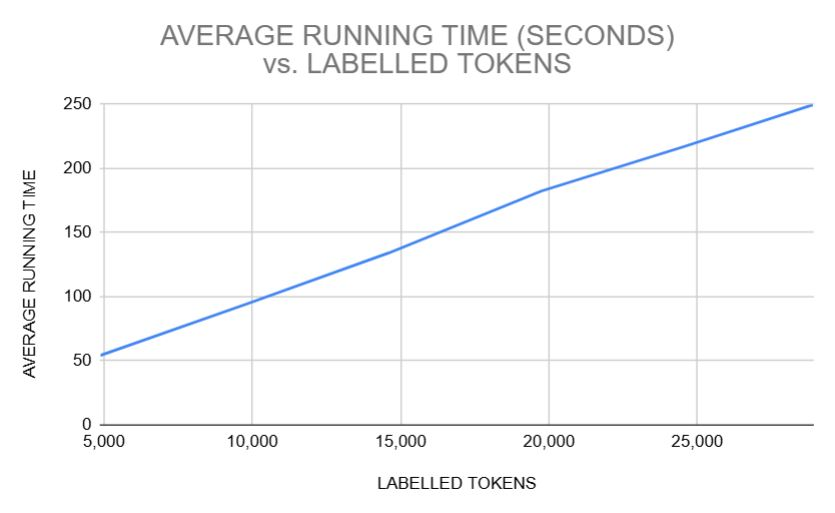
\includegraphics[scale=0.51]{images/Runtime Test Graph.JPG}
    \captionsetup{justification=centering}
    \caption{Graphical representation of the runtime test results of PANG-KAT.}
\end{figure}

The graphical representation of the runtime performance of PANG-KAT is directly proportional to the number of tokens labelled from its input text. In the runtime tests for NewPH-NLI, a significant portion of the runtime was observed to be attributed to the dictionary lookups performed during its identification of Tagalog NEs and MWEs. Therefore, the overall runtime increases in proportion to the frequency of Tagalog NEs and MWEs present in the input text and the number of dictionary lookups required to label them accurately.

\subsection {Discussion}

Given that the F1 score ranges from 0 to 1 {\cite{perEvalMetrics}}, with 1 indicating perfect classification performance for the model, the F1 scores achieved by PANG-KAT on the NewsPH-NLI dataset indicate good performance in accurately tokenizing and classifying Tagalog NEs and MWEs for both short and longer unit tokenization. \\

In the performance evaluation results, the deduction on PANG-KAT’s precision score was mainly caused by its heavy dependence on word patterns and its dictionary in classifying Tagalog NEs and MWEs. It lacked the ability to identify and understand deeper contextual meanings and relationships within words, which the testing revealed to also be crucial in improving the accuracy of its positive predictions and reduce false positives. For instance, PANG-KAT incorrectly identified "nakita kita" as a Tagalog MWE, given that it follows the structure of Tagalog repeating words. Similarly, it could misclassify the word "una" as an organization entity, confusing it with the acronym for the United Nationalist Alliance (UNA). This misclassification also occurred with words that may be used as names of a person (e.g., Precious, Miles, Win, Go, etc.). \\

On the other hand, the deduction on PANG-KAT’s recall score was mainly caused by other Tagalog NEs and MWEs that were not yet included in its dictionaries, which increases the rate of false negatives. Despite the researcher's efforts to broaden PANG-KAT’s dictionaries, numerous categories may still be added to each of PANG-KAT’s dictionaries. These include uncommon names for person entities, more specific locations (e.g., sitios, barrios, streets, puroks, etc.) for location entities, non-accredited and localized organizations for organization entities, and Taglish MWEs, which are currently lacking in available resources. \\

Moreover, PANG-KAT's dictionaries are primarily tailored to the Philippine context. This necessitates further expansion of its dictionaries (e.g., international names, locations, organizations, and MWEs) to broaden its application to international contexts. Lastly, PANG-KAT's heavy dependence on word patterns and its dictionary makes it unable to identify misspelled Tagalog NEs and MWEs, and improper usage of punctuation. It is recommended to integrate it with a preprocessing tool that would initially clean the data before tokenization to further improve the accuracy of its negative predictions and reduce false negatives. These further improvements for both precision and recall will also improve PANG-KAT’s resulting F1-score. \\

% CONCLUSION AND FUTURE WORK
\section{Conclusion and Future Work}
\subsection {Conclusion}

The main objective of this study is to develop PANG-KAT, a dedicated tokenizer for the Tagalog language that also incorporates the recognition of Tagalog named entities (NEs), multi-word expressions (MWEs), and Taglish tokenization, to develop a general tokenizer for real-world Tagalog language processing applications. This is to address the lack of language-specific NLP tools for Tagalog, despite being one of the most widely spoken languages in the Philippines. In this study, PANG-KAT was developed as a hybrid rule and dictionary-based tokenizer due to the lack of pre-annotated, publicly available resources for a machine-learning approach. \\

Through rigorous development and testing, PANG-KAT F1 scores exceeded 0.9 on both unit testing and external validation using the NewsPH-NLI dataset and Pilipino Star Ngayon articles for both short and longer unit tokenization. This indicates good performance in accurately tokenizing and classifying Tagalog NEs and MWEs. These results affirm the effectiveness of its rule set and dictionaries in capturing the patterns in Tagalog and Taglish texts. However, PANG-KAT’s heavy dependence on its rule set and dictionaries has its drawbacks, which make it unable to identify deeper contextual meanings and relationships within words, limited vocabulary coverage, and misclassifications caused by misspellings or improper usage of punctuation. These gaps suggest the need for further expansion of PANG-KAT’s dictionary to expand its application to broader contexts and its potential integration with other NLP components to improve its tokenization and classification capabilities. \\

\subsection {Recommendations}

Based on the identified gaps from the results of the study, the following are the recommendations of the researcher for further continuation of the study or other related research studies: \\

\begin{itemize}
  \item Expand the dictionary scope and coverage to improve recall and reduce false negatives. Additional categories for Tagalog NEs may also be included (e.g., events, objects, animals, etc.) depending on the type of data that needs to be tokenized.
  \item Integrate dedicated Tagalog pre-processing modules, particularly modules that correct misspellings and standardize punctuation to improve token classification accuracy and precision. Dedicated Tagalog pre-processing modules are important because of the presence of “jejemon” culture in the Philippines, which causes individuals to intentionally alter the spelling of words with specific symbols or alphanumeric characters. This is highly prevalent in informal contexts, particularly on social media, as observed in the TweetTaglish corpus. Thus, it is important to create a module for cleaning this type of data to allow its further NLP exploration.
  \item Integrate a dedicated Tagalog Part of Speech (POS) tagger, in an attempt to provide the tokenizer the ability to identify deeper contextual meanings and relationships within words, which would also improve token classification accuracy and precision.
  \item Develop a machine-learning-based tokenizer that could utilize the various manually annotated training and testing datasets of PANG-KAT.

\end{itemize}

% ACKNOWLEDGMENT
\section*{Acknowledgment}
This study would not have been possible without the unwavering trust and support of the important people in my life. To my family, your trust in me, in my capabilities and skills, was my greatest source of strength during times of self-doubt. To my friends, my emotional support, thank you for standing by me through the various difficult moments in university, for holding my trembling hands, and for reminding me that I was never alone. To my beloved partner, thank you for taking care of me during countless sleepless nights and making sure that I was eating properly. To those with whom I’ve parted ways along the journey, despite the endings, I would forever remain grateful for the lessons you’ve taught me and the memories we shared. \\

Above all, I thank God for surrounding me with such wonderful people who not only helped me complete this study but also shaped who I have become today. When I was feeling lost in life, my faith in You helped me believe that we can make every setback in life a setup for a meaningful comeback. \\

I also express my sincere gratitude to my adviser, Prof. Jaderick P. Pabico, for his time, knowledge, and guidance throughout this journey. It has been an honor to receive your trust and to work with you in this study. May this study be able to fulfill its purpose and be of use to those it aims to serve.

% BIBLIOGRAPHY
\printbibliography
% \nocite{*}

% BIOGRAPHY
\begin{biography}
[{\includegraphics[width=2.8cm,height=3cm]{./saavedra.eps}}]{\\ Justin Louis L. Saavedra}
is an undergraduate Computer Science student at the University of the Philippines Los Ba\~{n}os. He is also a proud member of the UPLB Computer Science Society (UPLB COSS).
\end{biography}


\end{document}
 
